\subsection{Experiments}
\begin{figure}[htb]
    \centering
    \subfigure[Feature alignment]{\label{fig-f}
        \centering
        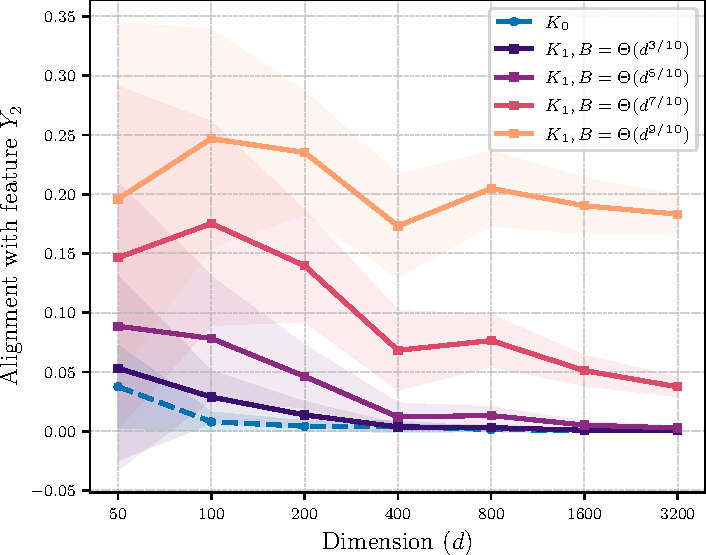
\includegraphics[width=0.35\textwidth, keepaspectratio]{figures/dimension_alignment.pdf}
    }
    \hspace{0.5cm}
    \subfigure[Test MSE]{\label{fig-t}
        \centering
        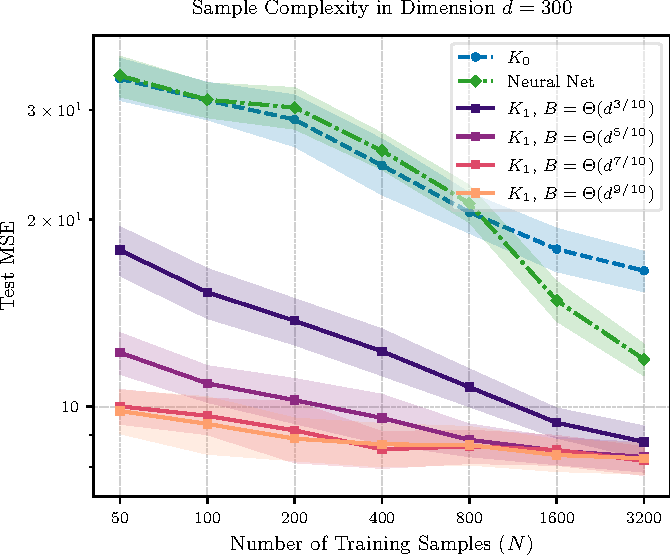
\includegraphics[width=0.35\textwidth,keepaspectratio]{figures/sample_complexity.pdf}
    }
    \caption{(a) Alignment with the directional feature $Y_2$. (b) Generalization performance at $d=300$.}
    \label{fig:exp}
\end{figure}

Here we provide numerical results to validate and understand our formal results. Over $10$ trials, with variance shown as shaded areas around the curves, we sample $\bm{Z} \in \mathbb{R}^{N \times d}$ with $\bm{z}_i \sim \mathcal{N}(0, \bm{I}_d)$, and compare the ReLU kernel $k_0$, the ReLU kernel $k_1$ from \cref{eq:relu-k1} and a two-layer ReLU MLP (width 400). In \cref{fig-f}, we compute the alignment $\langle \bm{v}_i^{\text{top}}, Y_2(\bm{Z}) \rangle$, where $\bm{v}_i^{\text{top}}$ is the lead eigenvector of the kernel matrices for $i \in \{0, 1\}$. As expected, the alignment for $k_1$ grows with $B$, while $k_0$ always remains near-zero. In \cref{fig-t} we track the Mean Squared Error ($d = 300$) on a test set of $600$ samples when learning $g(t) = 2t^2 + 3t + 4\sin(2t)$, comparing Kernel Ridge Regression and the network across varying training sample sizes $(N)$. We observe the network converging toward the spiked kernel’s performance; noting that while the kernels have privileged access to $\bm w^*$, the network must recover it from the data. Refer to \cref{app:experimental_details} for full details of the experimental setup.
